\documentclass[journal,12pt,twocolumn]{IEEEtran}
\usepackage{gensymb}
\usepackage{amssymb}
\usepackage[cmex10]{amsmath}
\usepackage{amsthm}
\usepackage[export]{adjustbox}
\usepackage{bm}
\usepackage{longtable}
\usepackage{enumitem}
\usepackage{mathtools}
 \usepackage{tikz}
\usepackage[breaklinks=true]{hyperref}
\usepackage{listings}
\usepackage{color}                                            %%
\usepackage{array}                                            %%
\usepackage{longtable}                                        %%
\usepackage{calc}                                             %%
\usepackage{multirow}                                         %%
\usepackage{hhline}                                           %%
\usepackage{ifthen}                                           %%
\usepackage{lscape}     
\usepackage{multicol}
\usepackage{graphicx}
% \usepackage{enumerate}

% \newcommand{\solution}{\noindent \textbf{Solution: }}
\title{Assignment II (ICSE Class 12 2019)}
\author{Kola Akshitha - AI21BTECH11017}
\begin{document}
\maketitle
\textbf{3b)} 
If $\sec^{-1}x = \csc^{-1}y$ , show that $\frac{1}{x^{2}}+\frac{1}{y^{2}} = 1$
\\
\textbf{Solution:}
 Given $\sec^{-1}x = \csc^{-1}y$\\
 The range of $\sec^{-1}x$ is $[0,\pi]-\lbrace\frac{\pi}{2}\rbrace$ \\
 The range of $\csc^{-1}y$ is $[-\frac{\pi}{2},\frac{\pi}{2}]-\lbrace0\rbrace$ \\
 Let  
\begin{align} 
 \sec^{-1}x = \csc^{-1}y = \theta \nonumber
 \\
\implies x = \sec\theta 
 \\
\implies y = \csc\theta 
 \end{align}
 From all the above statements we can conclude that range of $\theta$ is $\left(0,\frac{\pi}{2}\right).$ \\
 Then
 \begin{align}
 \frac{1}{x^{2}}+\frac{1}{y^{2}} = \frac{1}{\sec^{2}\theta}+\frac{1}{\csc^{2}\theta}
 \end{align}
 As
 \begin{align}
  \frac{1}{\sec\theta}&=\cos\theta \nonumber
  \\
   \frac{1}{\csc\theta}&=\sin\theta \nonumber
 \\
\implies \frac{1}{x^{2}}+\frac{1}{y^{2}}&=\cos^{2}\theta+\sin^{2}\theta
\\
&=1 \nonumber
 \end{align}
 Hence proved.
\begin{figure}[!ht]
 \centering
 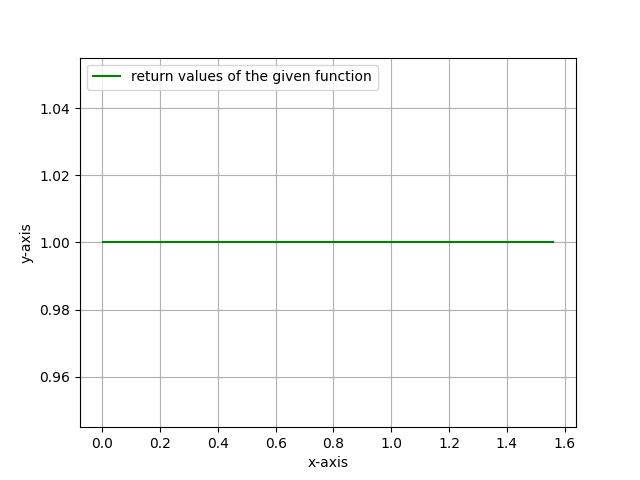
\includegraphics[width=\columnwidth]{code/figure2.png}
 \caption{proof for the condition}
 \label{fig-1}
 \end{figure}
 
 \end{document}
 
